\begin{document}
In this section, we will give an architecture overview of how the data gathering software should look and operate.
In \ref{fig:system_architecture}, we can see a general architecture. The platform is composed of two major modules:

\begin{figure}[htp]
    \centering
    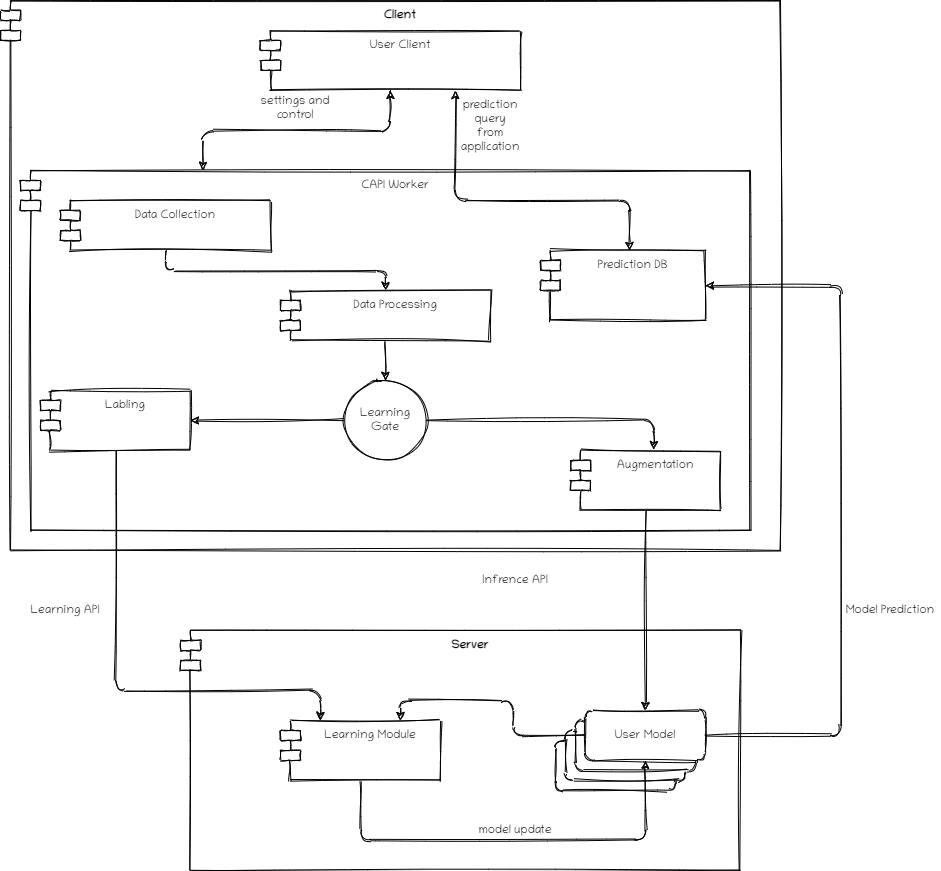
\includegraphics[width=12cm]{figures/platform_architecture.png}   
    \caption{The platform is composed of two major modules. The client runs on the user's computer,
        and is in charge of gathering data whether it is for learning or prediction.
        The server can be in a remote location and is in charge of the harder computations,
        such as training the personal models, and running the models on the user's data.}
    \label{fig:system_architecture} 
\end{figure}

\subsection{Client}
The client is also composed of two components. The first is the user client, which is the actual application the user can interact with.
This can come in different forms, but most likely a GUI that will summarize the worker's operations and control its settings,
in addition to using the predictions coming from the server in some way. The second component is the worker. This will most likely be a
separate process running on the user's computer, though it could also run on a different machine depending on the circumstances.
The worker is the mediator between the server, the user client, and the user himself (his data).

 
\begin{itemize}
    \item \emph{Data Collection} - The data collection module is straightforward. It collects the user's data that is needed for the model to make
        its predictions. This module needs to be very extensible, as different methods might require different data sources and variants.
    \item \emph{Data Processing} - The data processing module receives data from data collectors, it applies appropriate data processing to the data,
        such as normalization, scaling, and so on. It then passes the processed data to the next stage in the system.
    \item \emph{Learning Gate} - The learning gate is a simple construct tuned for each model or user. It simply decides when the model needs
        to continue its training. If it decides the model can make a prediction, the data from the Data Collector is passed to the
        Augmentation module. Otherwise, the data will be passed to the learning module.
    \item \emph{Labeling Module} - When the labeling module receives data, it will try to label it (usually by prompting the user).
        Once the data is labeled, it can be sent to the server to train the model. Again the module will be extensible,
        allowing different labeling options to be implemented.
    \item \emph{Augmentation Module} - When data reaches the augmentation module, it means that it needs to get to the server to make a prediction,
        the augmentation module has two goals:
        \begin{enumerate}[i]
            \item \emph{Augmentation} - We might want to apply additional augmentations to our data when training, or even at inference time,
                augmentations can be image rotations, flips, adding noise and so on.
            \item \emph{Reduction} - Some models can split in a way that allows one part to reduce the dimensionality of the data and the other to
                make a prediction using the data embedded in the reduced dimension. An excellent example of that is a CNN architecture with
                multiple pooling layers. Because the data is often not small, especially with images or videos, we prefer to run as
                much of the model as possible on the client. If we continue with the CNN example, the image will run through the model's
                first few layers. This will reduce the data's size. The data will be sent over the wire to the server,
                where the rest of the computation will complete. This separation might not always be possible, but when it is, it has the potential
                to save a lot of the time spent transferring the data over the wire.
        \end{enumerate}
    \item \emph{Prediction Database} - The prediction database contains the results of the prediction from the server.
        This is necessary because we might not want to use the results immediately, instead wait for when some event occurs
        (for example, when a news report comes in, the user client will query the
        database and check the user's current mood).
\end{itemize}
 

\subsection{Server}

The server is meant to perform the more expensive computations and will likely not be running on the client machine.
Though we do not disregard the possibility of the server running on the same machine as the client,
a perfect example is if we do not want any of the client's data moving through the internet. The server exposes two APIs:

 
\begin{itemize}
    \item \emph{Learning API} - the learning API receives requests from the client with labeled data.
        The data from the client is collected and then applied to the client's model during training runs.
    \item \emph{Inference API} - the inference API receives requests from the client with unlabeled data. After it passed through the augmentation module,
        the server runs the client's model on the data and returns the predictions to the client.
\end{itemize}
 

This paradigm, where each client has a personalized model on the server, can quickly get very expensive.
A few possible improvements can be running part of the model in the augmentation module on the client as discussed before,
Having parts of the model shared between clients. If we use the CNN example again, many of the features will be shared by all clients,
Furthermore, each client will have some additional features and maybe also individual FC layers.
If an ensemble method is used, some models may be shared between multiple or all clients.
 
\end{document}